\documentclass[12pt]{extarticle}
\usepackage[utf8]{inputenc}
\usepackage{cite}
\usepackage{graphicx}
\usepackage{appendix}



\title{Project Proposal: An Application That Does A Thing}
\author{Student McStudentface}
\date{October 2019}

\begin{document}

\maketitle

\section{Overview} \small
This is the overview. The overview should let the reader know that 
this document is describing a proposed application. It should also give
a brief overview of what the application is -- but not give away too much
information. Keep it brief. Lorem ipsum dolor sit amet, consectetur adipiscing elit, sed do eiusmod tempor incididunt ut labore et dolore magna aliqua. Ut enim ad minim veniam, quis nostrud exercitation ullamco laboris nisi ut aliquip ex ea commodo consequat. Duis aute irure dolor in reprehenderit in voluptate velit esse cillum dolore eu fugiat nulla pariatur. Excepteur sint occaecat cupidatat non proident, sunt in culpa qui officia deserunt mollit anim id est laborum \cite{fractalwiki}.

\section{Project Description} \small
This is the meat of your proposal. Here is where you describe the detailed 
features that you'd like to include in the application. There should be a few
mock-up images here \cite{vihart}. Lorem ipsum dolor sit amet, consectetur adipiscing elit, sed do eiusmod tempor incididunt ut labore et dolore magna aliqua. Ut enim ad minim veniam, quis nostrud exercitation ullamco laboris nisi ut aliquip ex ea commodo consequat. Duis aute irure dolor in reprehenderit in voluptate velit esse cillum dolore eu fugiat nulla pariatur. Excepteur sint occaecat cupidatat non proident, sunt in culpa qui officia deserunt mollit anim id est laborum.

\begin{figure}[!ht]
\centering
  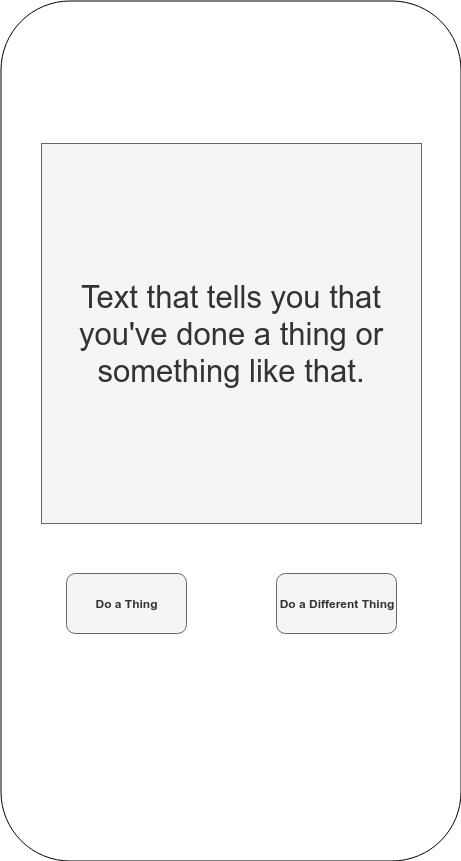
\includegraphics[width={0.2\linewidth}]{img/thing.jpg}
  \caption{A thing.}
  \label{fig:thing1}
\end{figure}

As you see in Fig. \ref{fig:thing1} you should include a basic mock-up of what your application will look like. This will help give the reader a better idea of exactly what you are proposing. It is also a good idea to include a flow-chart to show functionality. There's an example in Fig. \ref{fig:flowchart}. Lorem ipsum dolor sit amet, consectetur adipiscing elit, sed do eiusmod tempor incididunt ut labore et dolore magna aliqua. Ut enim ad minim veniam, quis nostrud exercitation ullamco laboris nisi ut aliquip ex ea commodo consequat. Duis aute irure dolor in reprehenderit in voluptate velit esse cillum dolore eu fugiat nulla pariatur. Excepteur sint occaecat cupidatat non proident, sunt in culpa qui officia deserunt mollit anim id est laborum.

\begin{figure}[!ht]
\centering
  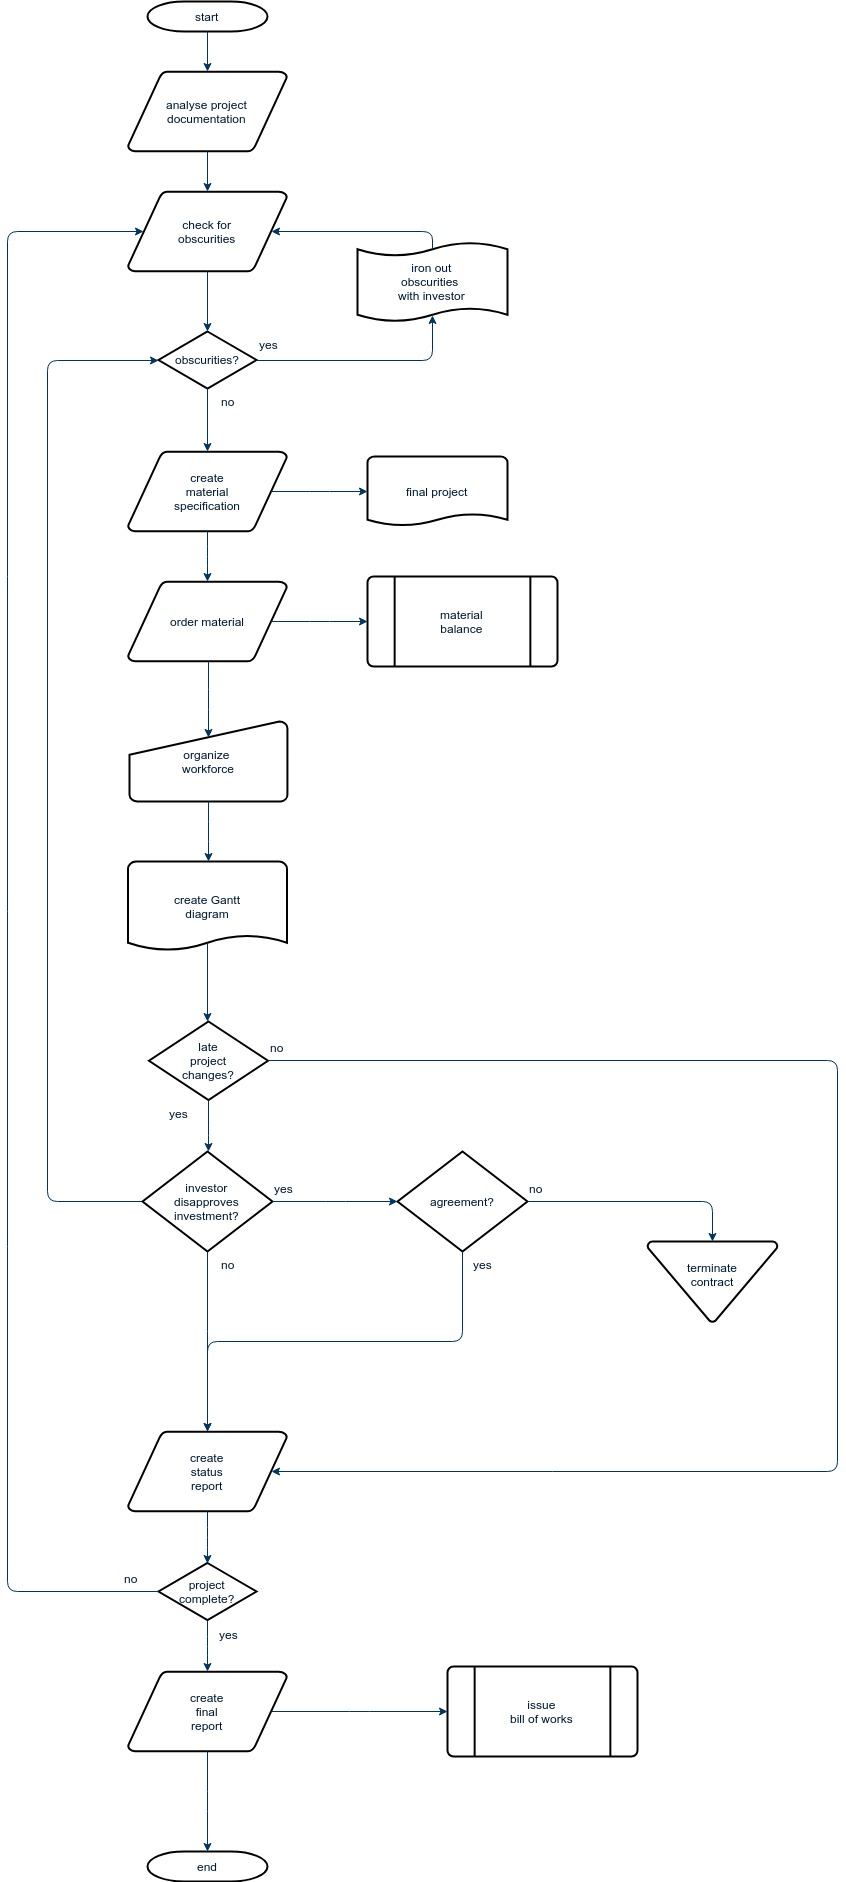
\includegraphics[width={0.2\linewidth}]{img/flowchart.jpg}
  \caption{A flowchart for the sake of a flowchart.}
  \label{fig:flowchart}
\end{figure}

The flowchart above is way too hard to read. You can change the size of an image by changing ``width'' inside the includegraphics tag. Lorem ipsum dolor sit amet, consectetur adipiscing elit, sed do eiusmod tempor incididunt ut labore et dolore magna aliqua. Ut enim ad minim veniam, quis nostrud exercitation ullamco laboris nisi ut aliquip ex ea commodo consequat. Duis aute irure dolor in reprehenderit in voluptate velit esse cillum dolore eu fugiat nulla pariatur \cite{higham1998handbook}. Excepteur sint occaecat cupidatat non proident, sunt in culpa qui officia deserunt mollit anim id est laborum.


\section{Technical Specifications}
This is where you will give the technical specifications of your project. For example, will you be using firebase or something like that? Lorem ipsum dolor sit amet, consectetur adipiscing elit, sed do eiusmod tempor incididunt ut labore et dolore magna aliqua. Ut enim ad minim veniam, quis nostrud exercitation ullamco laboris nisi ut aliquip ex ea commodo consequat. Duis aute irure dolor in reprehenderit in voluptate velit esse cillum dolore eu fugiat nulla pariatur. Excepteur sint occaecat cupidatat non proident, sunt in culpa qui officia deserunt mollit anim id est laborum.Lorem ipsum dolor sit amet, consectetur adipiscing elit, sed do eiusmod tempor incididunt ut labore et dolore magna aliqua. Ut enim ad minim veniam, quis nostrud exercitation ullamco laboris nisi ut aliquip ex ea commodo consequat. Duis aute irure dolor in reprehenderit in voluptate velit esse cillum dolore eu fugiat nulla pariatur. Excepteur sint occaecat cupidatat non proident, sunt in culpa qui officia deserunt mollit anim id est laborum.

\section{Time-line}
This section is really important. This is where you will give a list of milestones that you want to meet and when you will meet them by. Here is a list of milestones:
\begin{itemize}
	\item Milestone 1: Do a thing -- October 25th 2019
	\item Milestone 2: Do another thing -- November 1st 2019
	\item Milestone 3: Do a third thing -- November 20th 2019
	\item Milestone 4: Almost done -- November 29th 2019
    \item Milestone 5: Everything is finished -- December 12th 2019
\end{itemize}

Another great way to organize your project is do develop a Gantt chart (give it a google -- there's loads of documentation on Gantt charts). Fig. \ref{fig:gantt} shows an example of what a Gantt chart might look like. 

\begin{figure}[!ht]
\centering
  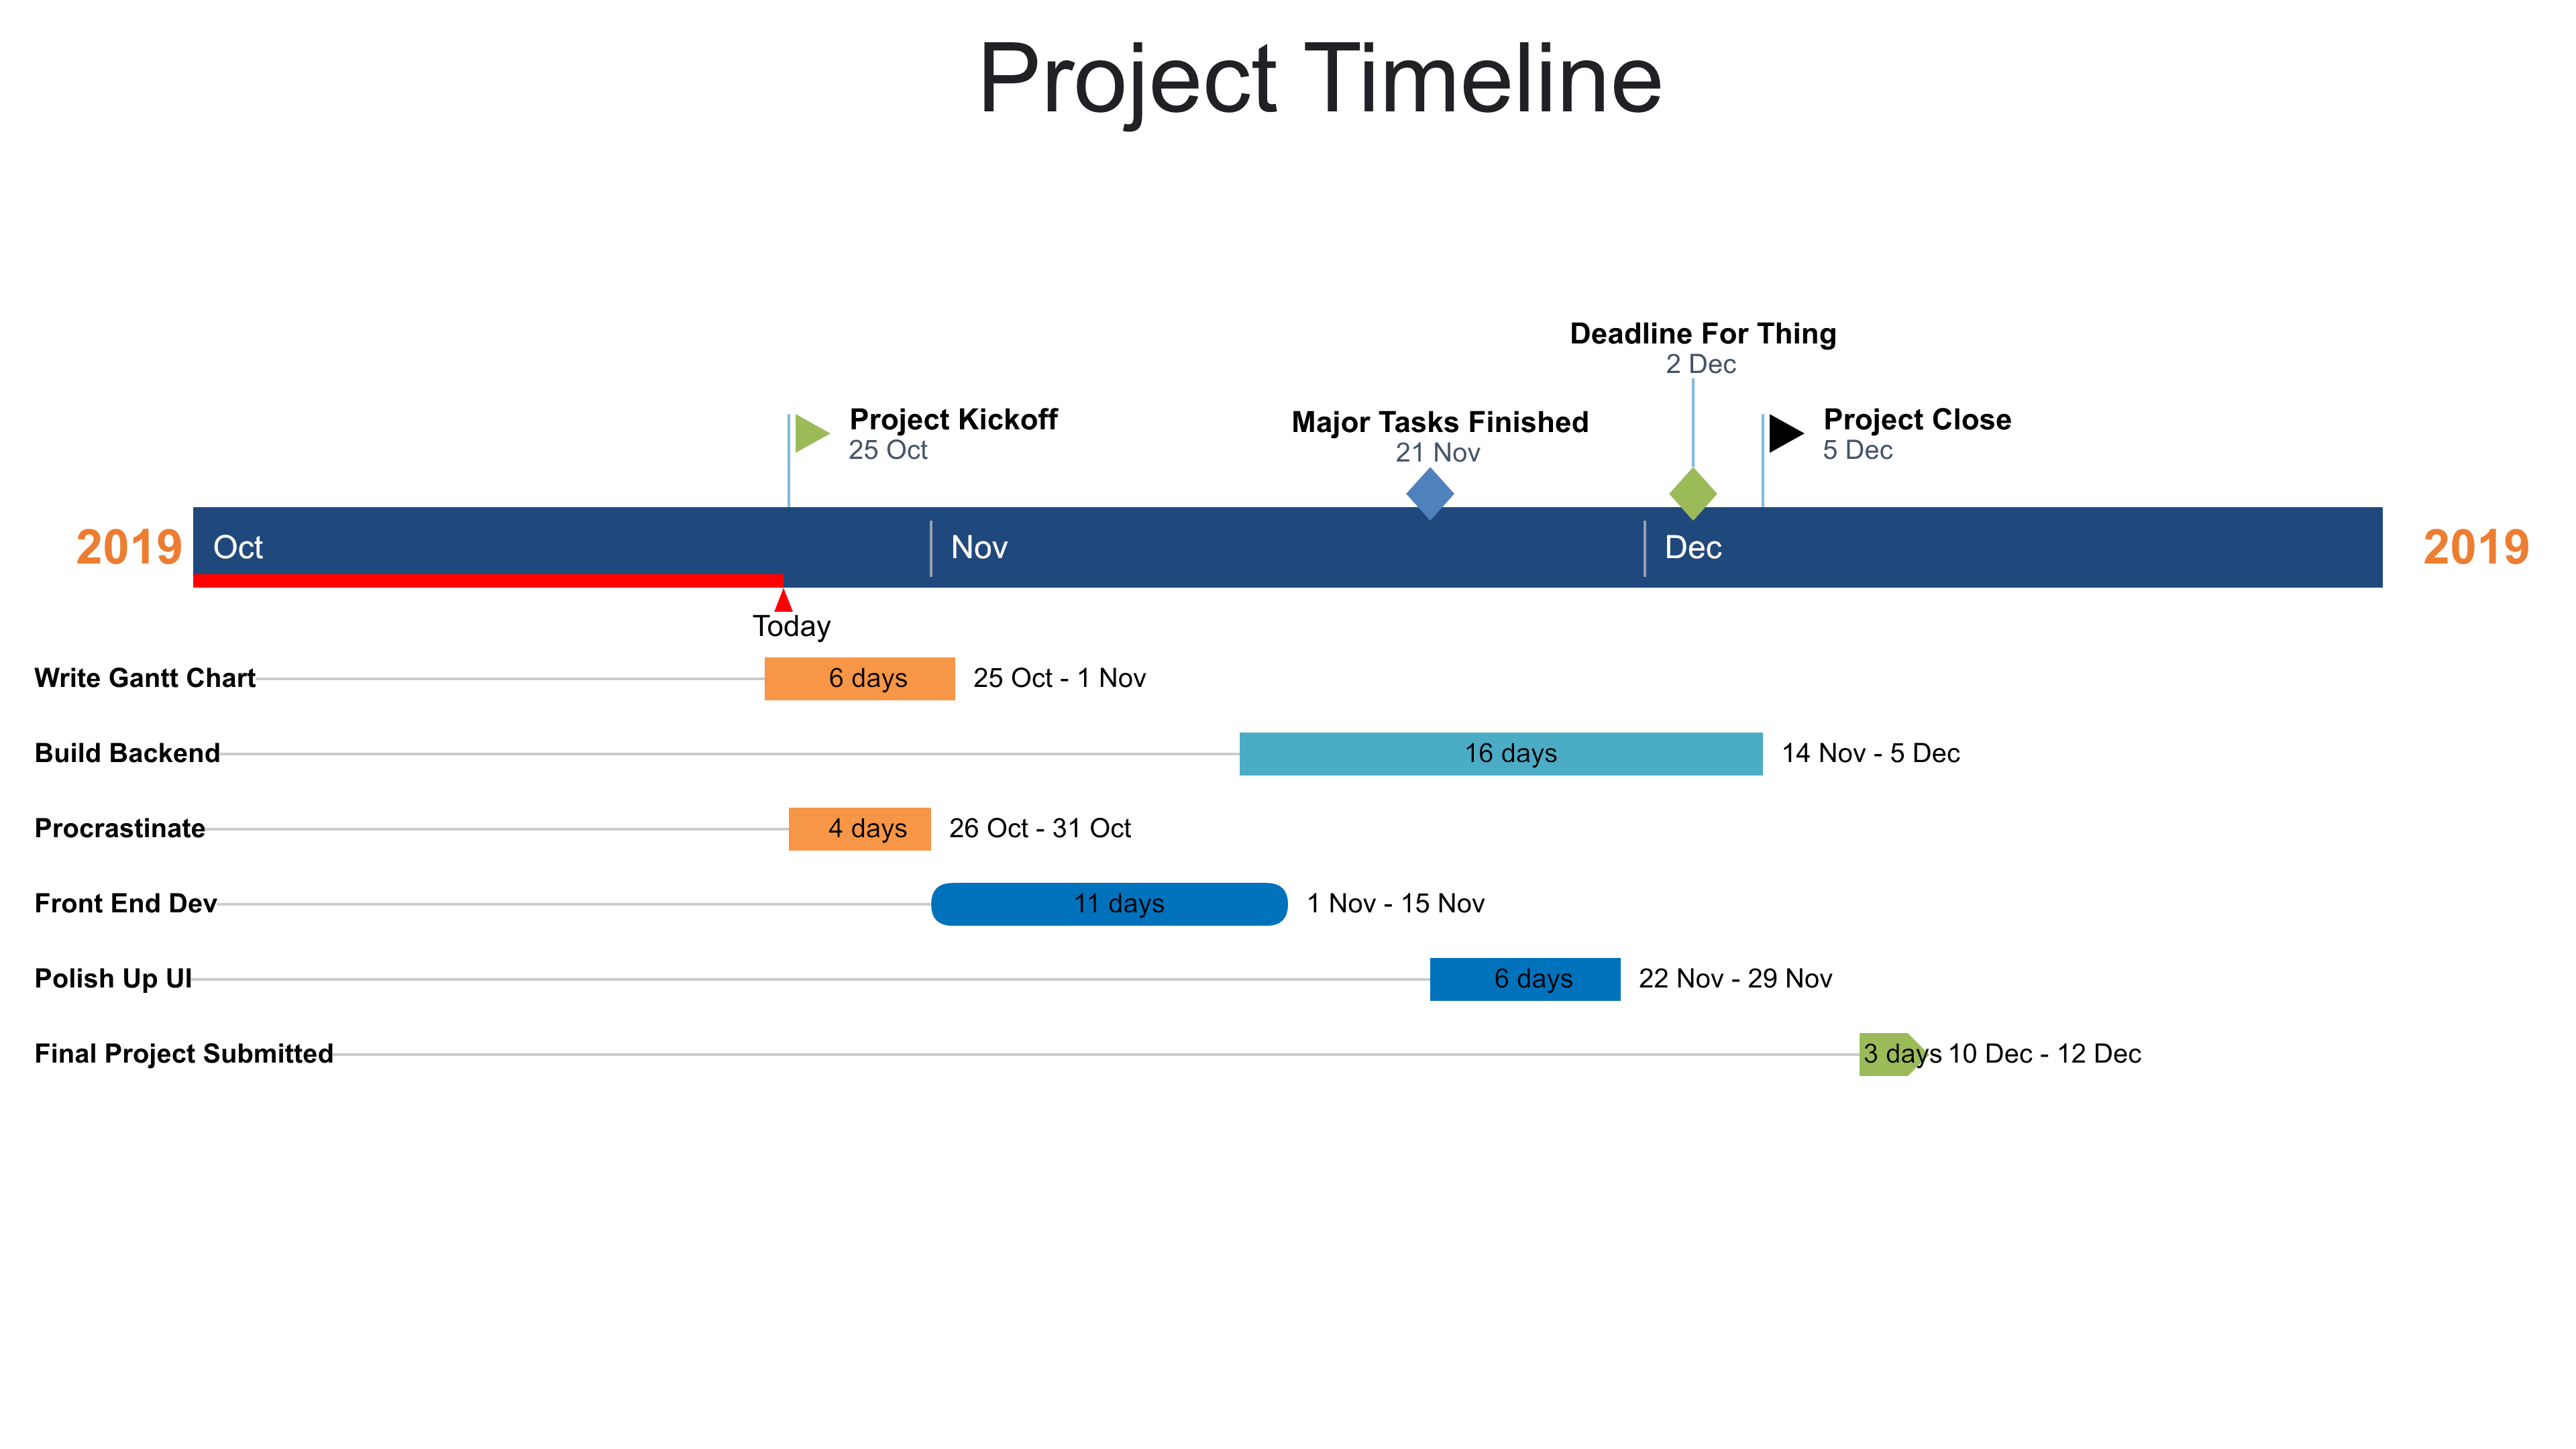
\includegraphics[width={\linewidth}]{img/gantt.png}
  \caption{This is a Gantt Chart. It's a great way to organize your project development!}
  \label{fig:gantt}
\end{figure}

Lorem ipsum dolor sit amet, consectetur adipiscing elit, sed do eiusmod tempor incididunt ut labore et dolore magna aliqua. Ut enim ad minim veniam, quis nostrud exercitation ullamco laboris nisi ut aliquip ex ea commodo consequat. Duis aute irure dolor in reprehenderit in voluptate velit esse cillum dolore eu fugiat nulla pariatur. Excepteur sint occaecat cupidatat non proident, sunt in culpa qui officia deserunt mollit anim id est laborum.Lorem ipsum dolor sit amet, consectetur adipiscing elit, sed do eiusmod tempor incididunt ut labore et dolore magna aliqua. Ut enim ad minim veniam, quis nostrud exercitation ullamco laboris nisi ut aliquip ex ea commodo consequat. Duis aute irure dolor in reprehenderit in voluptate velit esse cillum dolore eu fugiat nulla pariatur. Excepteur sint occaecat cupidatat non proident, sunt in culpa qui officia deserunt mollit anim id est laborum \cite{Linhart2014}.
\newpage 

\appendix
\section{Figures}
If you have any figures that you want to include that you couldn't fit in the rest of the document 
you will want to put them here. 

\begin{figure}[!h]
\centering
  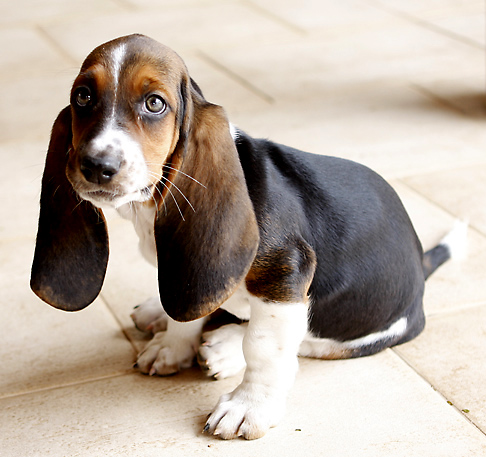
\includegraphics[width={0.4\linewidth}]{img/puppy1.jpg}
  \caption{Look at those stupid floppy ears!}
  \label{fig:puppy1}
\end{figure}

\begin{figure}[!h]
\centering
  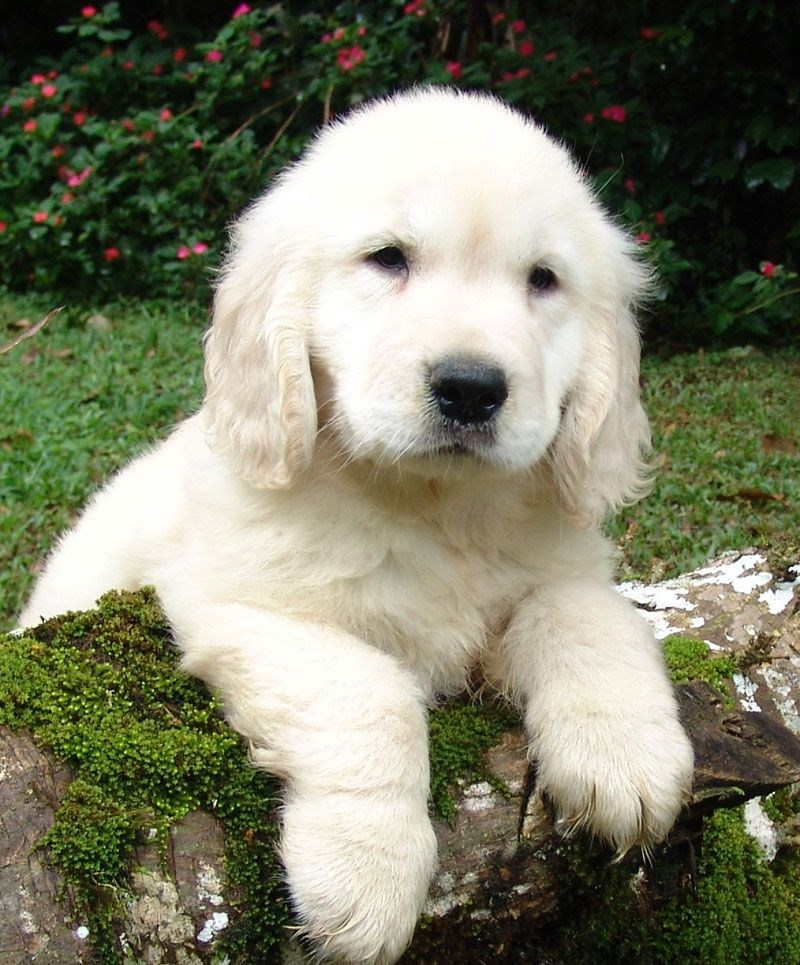
\includegraphics[width={0.4\linewidth}]{img/puppy2.jpg}
  \caption{I just wanna smooch that fuzzy little face!}
  \label{fig:puppy2}
\end{figure}

\begin{figure}[!h]
\centering
  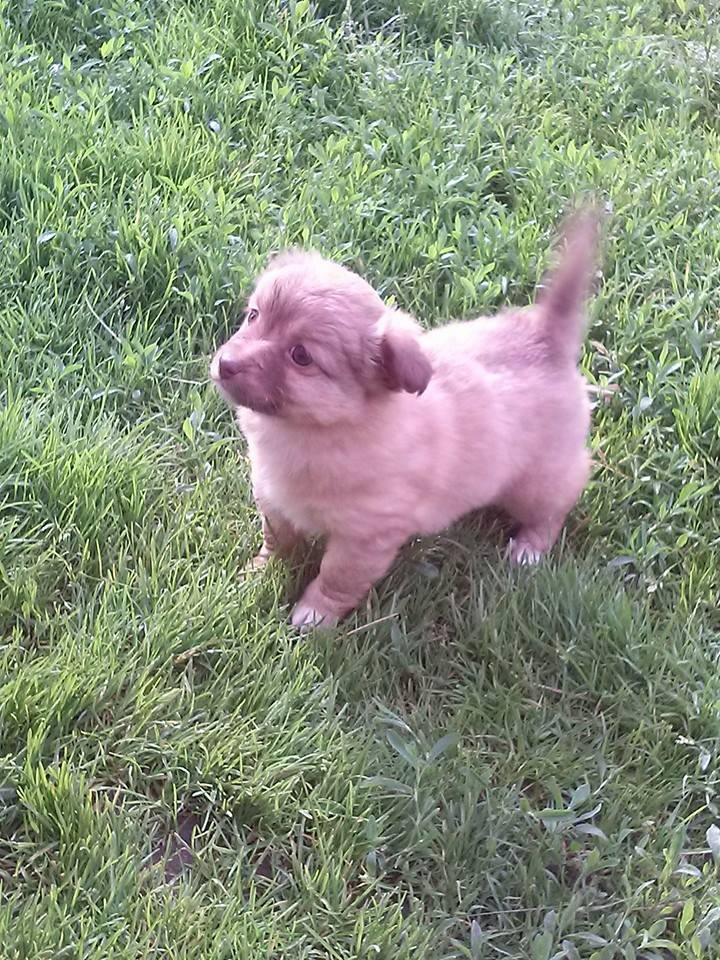
\includegraphics[width={0.4\linewidth}]{img/puppy3.jpg}
  \caption{It's so stupid cute!}
  \label{fig:puppy3}
\end{figure}
\newpage

\bibliographystyle{plain}
\bibliography{refs}

\end{document}
